%% Compile and read me!
\documentclass[a4paper,12pt]{article}
\pagestyle{empty}
\usepackage{color}
\usepackage[colorlinks=true,hyperfootnotes=false]{hyperref}
\usepackage{graphicx}
\usepackage[hypcap=true]{caption}
\usepackage[many]{tcolorbox}

\newtcolorbox{outerbox}[1]{%
    tikznode boxed title,
    enhanced,
    arc=0mm,
    interior style={white},
    attach boxed title to top left= {yshift=-\tcboxedtitleheight/2,xshift=5mm},
    fonttitle=\bfseries,
    colbacktitle=white,coltitle=black,
    boxed title style={size=normal,colframe=white,boxrule=0pt},
    title={#1}}


\newtcolorbox{innerbox}[1]{%
    enhanced,
    frame hidden,
    arc=2mm,
    interior style={lightgray},
    boxed title style={size=normal,colframe=white,boxrule=2pt}}

\begin{document}
\setlength{\parindent}{0cm}
\section*{NABU Paddle Support}
The NABU supports up to 4 paddles, 2 per controller port (8 if you populate the
missing components on your keyboard). The keyboard contains an 8 channel ADC that
is polled at the end of each keyboard matrix scan. If any value has changed since
the last scan, then they keyboard will send the updated paddle values to the NABU.
This is sent per controller port, so two values will get sent when a paddle on a
port changes its value. Each of the analog lines are pulled high with a 100k
resister.

\section*{Atari Paddle Modification}
Standard Atari paddles will not work with a NABU by default. This is due to
differences between how the NABU and Atari handle the analog input from paddles.

\bigskip

Unlike the NABU which uses a ADC to read an analog voltage level, the Atari paddles
generate a variable resistence which is then used to charge a capacitor. The time
it takes is used to determine the poisition of the paddle.

\bigskip

Fortunately it is easy enough to modify a stock atari paddle to work with the NABU.
If you open up your paddle you will note that one of terminals on the POT is floating.
This terminal needs to be connected to ground at which point a variable voltage will
be generated on the POT's wiper which can then be read by the NABU's ADC. This can be
easily achieved by connecting the unterminated terminal to the ground side of the paddle's
trigger button.

\smallskip

See Figure \ref{fig1:paddles} for the correct wiring diagram.

\bigskip

There is one other issue you will encounter with a stock Atari paddle. That is That
the POT used in them is nominally 1MOhm, which when combined with the 100k pullup
present on the analog lines will lead to a decidely non linear progression.

\medskip

A suiteable 100k drop in replacement POT is
\href{https://www.digikey.com/en/products/detail/cts-electrocomponents/450T328F104A1A1/4733114}{450T328F104A1A1}.

\pagebreak

\begin{figure}[h]
     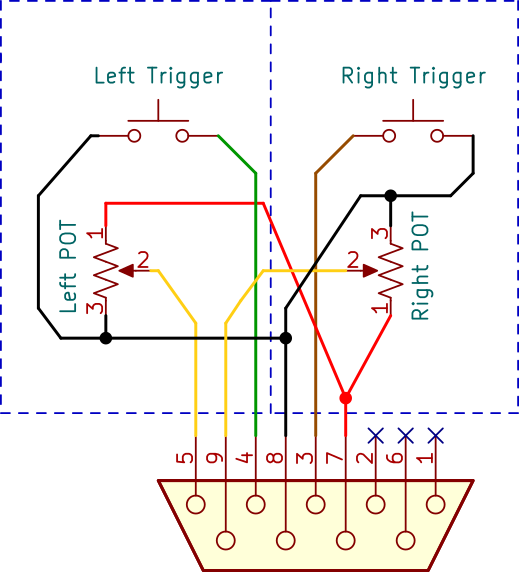
\includegraphics[width=\linewidth]{graphicx/paddles.png}
     \caption{Paddle wiring}
     \label{fig1:paddles}
\end{figure}

\pagebreak

\section*{Paddle Command Byte Format}
When sending the analog paddle data the keyboard will first send a command byte
over the serial connection to indicate which controller port the data belongs
to. Below are the command bytes used and which paddles data is being sent for:

\begin{itemize}
    \setlength\itemsep{-0.25em}
    \item \texttt{0x84 - paddles 1 and 2}
    \item \texttt{0x86 - paddles 3 and 4}
    \item \texttt{0x88 - paddles 5 and 6}\footnote{The ports for paddles 5-8 are unpopulated on the nabu keyboard}
    \item \texttt{0x8A - paddles 7 and 8}\footnotemark[\value{footnote}]
\end{itemize}


\section*{Paddle Data Byte Format}
Following each command byte there will be four data bytes. These four bytes
encode the current paddle values for the two paddles on the selected port. Each
byte represents a single nibble, with the least sigificant nibble being sent first.
The LSN will be encoded as "Cx" and the MSN is encoded as "Dx".
Where "x" is the value of that nibble.

\medskip

\begin{outerbox}{Example}
    \begin{innerbox}
        \texttt{\centering 0x84 0xCF 0xD4 0xC3 0xDF \par}
    \end{innerbox}
    {\centering $\downarrow$ \par}
    \begin{innerbox}
        \texttt{\centering Paddle 1: 0x4F, Paddle 2: 0xF3 \par}
    \end{innerbox}

\end{outerbox}

\end{document}
